\documentclass[12pt]{article}
\usepackage{amsmath}
\usepackage{hyperref}
\usepackage{verbatim}
\usepackage{graphicx}
\begin{document}
\begin{figure}[!htb]
  \center{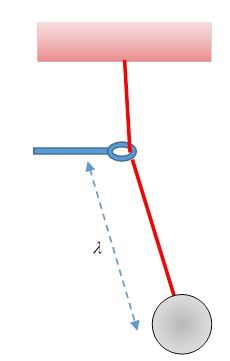
\includegraphics[scale=0.6]
    {variablepend.jpg}}
  \caption{\label{fig:my-label2} Variable Length Pendulum}
\end{figure}

The following argument is valid for any potential in which a trapped particle executes periodic motion of period $T$. If we also enforce that the potential depends on some variable parameter $\lambda$, which changes slowly ($T\frac{d\lambda}{dt}<<\lambda$). For a concrete example, we consider a pendulum of variable length: Fig. \ref{fig:my-label2}.

If $\lambda$ were fixed, both the period $T$ and the energy $E$ would be constant, but in general, the variable length exchanges energy with the system and thus varies both quantities. As explained in this \href{https://physics.stackexchange.com/questions/83541/when-does-the-total-time-derivative-of-the-hamiltonian-equal-its-partial-time-de}{Stack Exchange} post, when the path of satisfies Hamilton's equations (which would be the case in this pendulum example):
\begin{equation}\label{HamEQ}
\begin{split}
\dot{q}(t)=\frac{\partial H}{\partial p}(q(t),p(t),t)\\
\dot{p}(t)=-\frac{\partial H}{\partial q}(q(t),p(t),t)
\end{split}
\end{equation}
the full time derivative of the Hamiltonian is given by the partial time derivative of the Hamiltonian:
\begin{equation}\label{HamPartialt}
\frac{d H}{dt}=\frac{\partial H}{\partial t}
\end{equation}
For the case of the variable length pendulum, $H(q,p;\lambda)$, where $;$ is denoting what are parameters, and what are variables, see \href{https://www.mathsisfun.com/definitions/parameter.html}{mathisfun} for a painless explanation of this notation. We can use the chain rule on \eqref{HamPartialt} to obtain
\begin{equation}\label{HamChainRule}
\frac{dE}{dt}=\frac{\partial H}{\partial \lambda}\frac{d\lambda}{dt}
\end{equation}
where the time derivatives of $p(t)$ and $q(t)$ cancel as explained in the above Stack Exchange link. Note that it was assumed that the system is such that the Hamiltonian is equivalent to the total energy of the system. Since $\lambda$ varies slowly, if we average \ref{HamChainRule} over one period $\frac{d\lambda}{dt}$ is unaffected, and the equation becomes:
\begin{equation}\label{TimeAvgChain}
\overline{\frac{dE}{dt}}=\overline{\frac{\partial H}{\partial \lambda}}\frac{d\lambda}{dt}
\end{equation}
Where
\begin{equation}\label{TimeAvgHam}
\overline{\frac{\partial H}{\partial \lambda}}=\frac{1}{T}\int_0^T\frac{\partial H}{\partial\lambda}dt
\end{equation}
Due to Hamilton's equations \eqref{HamEQ} $dt=\frac{dq}{(\partial H)/\partial p)_{\lambda}}$ and the period becomes
\begin{equation}\label{Period}
T=\int_0^Tdt=\oint \frac{dq}{(\partial H/\partial p)}
\end{equation}
plugging \eqref{Period} into \eqref{TimeAvgChain} we obtain
\begin{equation}\label{TimeAvgChainInt}
\overline{\frac{dE}{dt}}=\frac{d\lambda}{dt}\frac{\oint \frac{(\partial H/\partial\lambda)dq}{\partial H/\partial p}}{\oint\frac{dq}{(\partial H/\partial p)_{\lambda}}}
\end{equation}
Since $E$ and $\lambda$ both are varying slowly, over a single cycle they can be considered constant and then at a point $q$, $p=p(q;E,\lambda)$, thus regarding $E$ and $\lambda$ as constant, independent parameters.

We can now partially differentiate $H(q,p,\lambda)=E$ with respect to $\lambda$ while keeping $E$ constant. This yields:
$$\frac{\partial H}{\partial \lambda}+\frac{\partial H}{\partial p}\frac{\partial p}{\partial \lambda}=0$$
or
\begin{equation}\label{ConstEp}
\left(\frac{\partial p}{\partial \lambda}\right)_E=-\frac{\partial h/\partial\lambda}{\partial H/\partial p}
\end{equation}  
plugging \eqref{ConstEp} into \eqref{TimeAvgChainInt} we get
\begin{equation}\label{TimeAvgChainInt2}
\overline{\frac{dE}{dt}}=-\frac{d\lambda}{dt}\frac{\oint (\partial p/\partial\lambda)_Edq}{\oint(\partial p/\partial E)_{\lambda}dq}
\end{equation}
Where $1/(\partial H/\partial p)_{\lambda}=(\partial p/\partial E)_{\lambda}$. We can rearrange \eqref{TimeAvgChainInt2} to get:
\begin{equation}\label{TimeAvgChainInt3}
\oint\left[ \left(\frac{\partial p}{\partial E}\right)_{\lambda}\overline{\frac{dE}{dt}}+\left(\frac{\partial p}{\partial \lambda}\right)_E\frac{d\lambda}{dt}\right]dq=0
\end{equation}
\eqref{TimeAvgChainInt3} can be written as $\overline{\frac{dI}{dt}}=0$ where
\begin{equation}\label{adiaInvar}
I=\oint p(q,\lambda,E)dq
\end{equation}
Where $I$ is the adiabatic invariant and the general form of the action integral. The slower the cycle we are concerned with is in relation to the change in the parameter, the less accurate conservation is. This is actually the lowest order approximation to a Poincare invariant. 
\subsubsection{First Adiabatic Invariant ($\mu$ Conservation)}\label{subsecfiradia}
Magnetic moment conservation is useful because it establishes a relationship between the perpendicular kinetic energy and the magnetic field. In the case of a magnetic field varying slowly in comparison with the gyrofrequency of the trapped particle, we can replace $p$ and $q$ in \eqref{adiaInvar} with $mv_{\perp}r_L$ and $\phi$ respectively. In this case, $\phi$ is the gyrophase of the particle, it varies from $0$ to $2\pi$ over the course of the particle's gyromotion. With that in mind, \eqref{adiaInvar} becomes:
\begin{equation}\label{gyroint}
I=\oint mv_{\perp}r_Ld\phi
\end{equation}
taking advantage of $\omega r=v$ and centripetal acceleration with the Lorentz equation, we integrate and get
\begin{equation}\label{firstadia}
I=\frac{2\pi}{q}\frac{m^2v_{\perp}^2}{B}=\frac{4\pi}{q}\frac{W_{\perp}}{B}\propto\mu
\end{equation}
So, with sufficiently slow $B$ variation, $\mu$ is a constant. 
\subsubsection{Second Adiabatic Invariant}\label{subsecsecadia}
Using \eqref{adiaInvar}, with generalized momentum $Mv_{\parallel}$ and generalized position as the distance along the mirror axis, we get the second adiabatic invariant:
\begin{equation}\label{secondadia}
J=\oint Mv_{\parallel}dz
\end{equation}
The following is a slightly reworded excerpt from from \href{https://farside.ph.utexas.edu/teaching/plasma/lectures/node24.html}{Fitzpatrick}: this invariant is associated with the periodic bouncing motion of a particle trapped between two mirror points on a magnetic field line. The value is only conserved if the bounce time is much smaller than the timescale at which the magnetic field varies. The invariance of $J$ is very important for charged particle dynamics in Earth's inner magnetosphere. This is because Earth's magnetic field is distorted from pure axisymmetry due to the action of the solar wind. Thus, there is no immediate reason to believe that the particle will return to its original trajectory after making the full rotation around Earth. In other words, a particle may well end up on a different field line after returning to its original azimuthal angle. However, at a given azimuthal angle, each field line has a different length between mirror points, and a different variation of the field strength for a particle with given energy and magnetic moment. Thus, each field line has a different $J$ value, and if $J$ is conserved, it means the particle must stay on the same field line throughout its motion. In other words, the conservation of $J$ prevents charged particles from spiraling radially in or out of the Van Allen belts as they rotate around Earth. This helps to explain the persistence of these belts. Note: A Van Allen belt is a zone of energetic charged particles, most of which originate from solar wind, that are captured by and held around a planet by that planet's magnetosphere. 

\textbf{Example}:

\vspace{1mm}
What happens when a ball elastically bounces between two parallel walls which are slowly closing in. Assume no gravity
\vspace{1mm}

As the walls are closing in slowly, we can assume that the second adiabatic invariant is conserved, so
$$J=\oint mv_{\parallel}dz=const$$
If we look at orders of magnitude we get
$$J~mv_{\parallel}L=const$$
Where $L$ is the distance between the walls. $m$ is constant and $L$ is decreasing, so to keep $J$ constant $v_{\parallel}$ must increase as the walls close in. So, the kinetic energy is increasing.
\end{document}